\section{PlanesQML}

The last of the 3 Qt based GUIs is PlanesQML. This uses QML, a declarative language similar to html to create the graphical interfaces.

\subsection{Main Window}

The main.cpp for the project looks as follows:

\begin{lstlisting}
	QGuiApplication app(argc, argv);
	QQmlApplicationEngine engine;
	
	PlaneGameQML planeGame;
	PlaneGridQML player_pgq(&planeGame, planeGame.playerGrid());
	PlaneGridQML computer_pgq(&planeGame, planeGame.computerGrid());
	player_pgq.initGrid();
	computer_pgq.initGrid();
	
	engine.rootContext()->setContextProperty("PlayerPlaneGrid", &player_pgq);
	engine.rootContext()->setContextProperty("ComputerPlaneGrid", &computer_pgq);
	engine.rootContext()->setContextProperty("PlaneGame", &planeGame);
	engine.load(QUrl(QStringLiteral("qrc:/main.qml")));
\end{lstlisting}

The QML interpreting engine is define by an object of the type QQmlApplicationEngine. Our application implements everything in QML except for the game engine, which is implemented in C++. In order to be able to reference the C++ objects in QML, two wrapper classes were created: PlaneGameQML and PlaneGridQML. 

Here below is the header file for PlaneGameQML:

\begin{lstlisting}

class PlaneGameQML : public QObject
{
	Q_OBJECT
public:
	PlaneGameQML();
	~PlaneGameQML();

public:
	Q_INVOKABLE void doneEditing();
	Q_INVOKABLE inline int getPlayerMoves() { return m_Stats.m_playerMoves; }
	Q_INVOKABLE inline int getPlayerHits() { return m_Stats.m_playerHits; }
	Q_INVOKABLE inline int getPlayerDead() { return m_Stats.m_playerDead; }
	Q_INVOKABLE inline int getPlayerMisses() { return m_Stats.m_playerMisses; }
	Q_INVOKABLE inline int getPlayerWins() { return m_Stats.m_playerWins; }
	Q_INVOKABLE inline int getComputerMoves() { return m_Stats.m_computerMoves; }
	Q_INVOKABLE inline int getComputerHits() { return m_Stats.m_computerHits; }
	Q_INVOKABLE inline int getComputerDead() { return m_Stats.m_computerDead; }
	Q_INVOKABLE inline int getComputerMisses() { return m_Stats.m_computerMisses; }
	Q_INVOKABLE inline int getComputerWins() { return m_Stats.m_computerWins; }
	
	Q_INVOKABLE void startNewGame();
	
	inline PlaneGrid* playerGrid() { return mRound->playerGrid(); }
	inline PlaneGrid* computerGrid() { return mRound->computerGrid(); }

signals:
	void guessMade(const GuessPoint& gp);
	void computerMoveGenerated(const GuessPoint& gp);    
	void updateStats();
	void roundEnds(bool isPlayerWinner);
	void resetGrid();

public slots:
	void statsUpdated(const GameStatistics& stats);
	void receivedPlayerGuess(const GuessPoint& gp);

private:
	//The controller object
	PlaneRound* mRound;
	GameStatistics m_Stats;
};

\end{lstlisting}

Observe that the class derives from QObject and that some methodes are declared using the Qt macro Q\_INVOKABLE. This allows the methods to be accessible from the QML code. PlaneGridQML has a header file with the same characteristics.

In order to register the C++ object with the QML engine one uses the setContextProperty() function as shown above.

By using the function load() one can define the start qml object for the project: main.qml

\begin{lstlisting}

Window {
	visible: true
	width: 1000
	height: 700

Row {
	anchors.fill: parent
	LeftPane {
		id: leftPane
	}
	RightPane {
		id: rightPane
	}
	}
}
\end{lstlisting}

This defines a window with 100 X 700 size composed of two subobjects: LeftPane and RightPane, which play similar roles as in PlanesGraphicsScene.

\begin{figure}[h]
	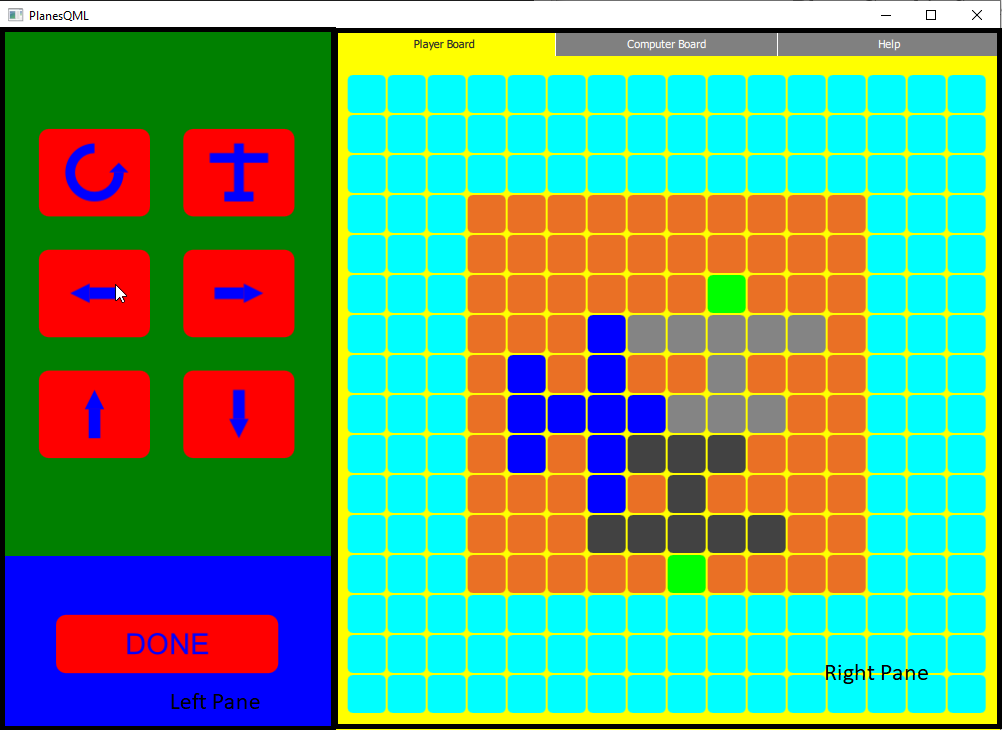
\includegraphics[width = \textwidth]{PlanesQML_BoardEditing_WidgetNames.png}
	\caption{Simplified Layout of PlanesQML}
	\label{fig:planesqml_boardediting_widgetnames}
\end{figure}

\subsection {LeftPane}

The QML code for the left pane is as follows:

\begin{lstlisting}
Rectangle {
	width: parent.width/3
	height: parent.height
	property alias currentTab : stack.currentIndex
	
	StackLayout {
		id: stack
		width: parent.width
		height: parent.height
		
		currentIndex: 1
		GameStatistics {
			id: roundTab
		}
		BoardEditorControls {
		}
		Rectangle {
			id: startTab
			color: "blue"
		}
	}
	
	Connections {
		target: PlaneGame
		onUpdateStats: {
			roundTab.playerMoves = PlaneGame.getPlayerMoves()
			roundTab.playerHits = PlaneGame.getPlayerHits()
			roundTab.playerMisses = PlaneGame.getPlayerMisses()
			roundTab.playerDead = PlaneGame.getPlayerDead()
			roundTab.playerWins = PlaneGame.getPlayerWins()
			roundTab.computerMoves = PlaneGame.getComputerMoves()
			roundTab.computerHits = PlaneGame.getComputerHits()
			roundTab.computerMisses = PlaneGame.getComputerMisses()
			roundTab.computerDead = PlaneGame.getComputerDead()
			roundTab.computerWins = PlaneGame.getComputerWins()
		}
	}
}
\end{lstlisting}

It contains a start tab, a board editing tab, containing the buttons to position the planes board, and a game tab, displaying computer and player game statistics during the game. These objects are grouped under a stack layout, that is a widget containing more superimposed widgets. For an explanation of the Connections element see \ref{qml:connections}.

\subsubsection {BoardEditing Tab}

The board editing tab contains buttons to position the planes on the game board. Here below is the implementation for the plane rotation button.


\begin{lstlisting}
import "ButtonPaintFunctions.js" as PaintFunctions

Rectangle {
	id: back
	color: "red"
	radius: 10
	
	Canvas {
		width: back.width
		height: back.height
		
		onPaint: {
			var ctx = getContext("2d")
			PaintFunctions.rotateButton(ctx)
		}
	}
	
	MouseArea {
		width: parent.width
		height: parent.height
		onClicked: {
		//console.log("Rotate clicked")
		anim.start()
		PlayerPlaneGrid.rotateSelectedPlane();
		PlayerPlaneGrid.verifyPlanePositionValid()
		}
	}
	
	SequentialAnimation {
		id: anim
		PropertyAnimation { target: back; property: "color"; to: "green"; duration: 50 }
		PropertyAnimation { target: back; property: "color"; to: "red"; duration: 50 }
		}
}
\end{lstlisting}

The button is encapsulated inside a rectangle with rounded corners (see attribute radius of the QML object Rectangle). It contains a canvas element which defines the design of the button. This is accomplished in the signal handler onPaint. In order to react to click events a MouseArea element is used. To graphically represent the click event a small animation is created - see \ref{qml:animation}.

One remarks here that the buttons are not standard buttons as for example the Qt Widgets buttons that we used in PlanesWidgets or PlanesGraphicScene. They are completely custom defined, proving the flexibility and resourcefullness of QML.

\subsubsection {Game Tab}


The GameTab contains the statistics for both the computer and the player. The data is displayed with a ColumnLayout (its elements are displayed all one under the other in a single column), that contains labels (texts) and tables configured with GridLayout layouts.

For example the stats for the player are displayed with the following code:

\begin{lstlisting}
GridLayout {
	columns: 2
	columnSpacing:  gameStats.width/10
	anchors.margins: gameStats.width/10
	
	Label {
		font.pixelSize: gameStats.textSize
		text: "Number of moves"
		color: gameStats.textColorGame
	}
	Label {
		font.pixelSize: gameStats.textSize
		id: noMovesComputer
		text: gameStats.computerMoves
		color: gameStats.textColorGame
	}
	Label {
		font.pixelSize: gameStats.textSize
		text: "Number of misses"
		color: gameStats.textColorGame
	}
	Label {
		font.pixelSize: gameStats.textSize
		id: noMissesComputer
		text: gameStats.computerMisses
		color: gameStats.textColorGame
	}
	Label {
		font.pixelSize: gameStats.textSize
		text: "Number of hits"
		color: gameStats.textColorGame
	}
	Label {
		font.pixelSize: gameStats.textSize
		id: noHitsComputer
		text: gameStats.computerHits
		color: gameStats.textColorGame
	}
	Label {
		font.pixelSize: gameStats.textSize
		text: "Number of planes guessed"
		color: gameStats.textColorGame
	}
	Label {
		font.pixelSize: gameStats.textSize
		id: noGuessedComputer
		text: gameStats.computerDead
		color: gameStats.textColorGame
	}
}
\end{lstlisting}

The GridLayout contains a list of Label sub-objects. The attribute columns specifies that the labels are to be displayed in two columns.

\subsubsection {Start New Game Tab}

The start new game tab is defined together with the game tab in the GameStatistics.qml source file and consists mainly of a button which when clicked triggers the start of a new game round.

\subsection {RightPane}

The RightPane contains the two important game boards and a help page glued together with the StackLayout. The most important part of the RightPane and of the application itself are the two game boards, defined in the QML object GenericBoard.

The three main components of the right pane and their grouping in a StackLayout are shown below:

\begin{lstlisting}
StackLayout {
	id: stackLayout
	anchors.top: bar.bottom
	currentIndex: bar.currentIndex
	width: parent.width
	height: parent.height - bar.height
	
	GenericBoard {
		boardModel: PlayerPlaneGrid
		id : playerBoard
		isComputer: false
	}
	
	GenericBoard {
		boardModel: ComputerPlaneGrid
		id : computerBoard
		isComputer: true
	}
	
	Rectangle {
		color: 'yellow'
		width: parent.width
		height: parent.height
		
		ListView {
			anchors.fill : parent 
			model: HelpPageModel {}
			delegate: Text {
				text: "<h3> "+ name +  "</h3>" + " <p> " + content + " </p>"
				width: parent.width - 10
				x: 5
				wrapMode: Text.WordWrap
			}
			clip: true
			ScrollBar.vertical: ScrollBar {}
		}
	}
}
\end{lstlisting}

The GenericBoard objects are custom objects defined in the application. Their two most important properties are boardModel, which represents the data model for the board, and the boolean isComputer, which specifies whether the board corresponds to a computer or a player.

The core of the generic board is the GridView which is another one of QML's view model classes - see \ref{qml:gridview}


\subsection {QML Concepts}

\subsubsection {QML Objects}

QML objects can be declared with the following syntax: 

\begin{lstlisting}

ObjectTypeName {

	attribute1: value1
	attribute2: value2
	..................
}

\end{lstlisting}

One such example is the main window object:

\begin{lstlisting}

Window {
	visible: true
	width: 1000
	height: 700
}

\end{lstlisting}

\subsubsection {QML Object property}

In addition to standard attributes one can declare custom attributes for a QML object, the so called properties. Properties are used for example in GenericBoard.qml:

\begin{lstlisting}
	property int gridSquaresOnLine: 10
	property int gridBorder: 3
	property string colorBackground: "yellow"
	property string colorBoard: "#ea7025"
	property string colorBorder: "aqua"
	property int cellSize : (Math.min(width, height) - 20) / (board.gridSquaresOnLine + 2 * board.gridBorder)
	property int spacing: 2
	property variant boardModel: ComputerPlaneGrid
	property bool isComputer: true
\end{lstlisting}

Each property has a type assigned to it and can be initiliazed with an expression depending on other properties and attributes.

\subsubsection {QML Object property aliases}

A property alias is a property which is a reference to another property. For example in the definition of the LeftPane we have the property alias currentTab which is a reference to the attribute stack.currentIndex, the index of the active view in the StackLayout of the LeftPane. 

\subsubsection {QML Subobjects}

In a QML application a hierarchy of objects and sub-objects exists. This hierarchy has a single root object. In our case it is the main window object. The other objects are all sub-objects of this main object. 
For example LeftPane and RightPane are sub-objects of the main window. 

\subsubsection {QML Layouts}

One type of QML objects are layouts. For example Row in the main window allows to display the LeftPane and RightPane in the same horizontal row. Other examples of layouts used in this application are: StackLayout (used in the LeftPane), ColumnLayout and GridLayout (used in GameStatistics)

\subsubsection {QML GridView} \label{qml:gridview}

The core of the game implementation is the display of the game board inside of a GridView layout using as model C++ functionality from the game engine.

\begin{lstlisting}
GridView {
anchors.centerIn: parent
width: parent.width
height: parent.height
cellWidth: board.cellSize
cellHeight: board.cellSize
flow: GridView.FlowTopToBottom


model: board.boardModel
delegate: Rectangle {
	width: board.cellSize
	height: board.cellSize
	color: board.colorBackground
	Rectangle {
	
	function squareColor() {
		if (board.state == "GameNotStarted" )
			return planeColorData;
		if (!isComputer)
			return planeColorData;
		if (boardData == 1)
			return planeColorData;
		return "#ea7025"; //TODO: to change this
	}
	
	anchors.centerIn: parent
	width: parent.width - board.spacing
	height: parent.height - board.spacing
	radius: 5
	color: squareColor()
	Canvas {
		anchors.fill: parent
		width: parent.width
		height: parent.height
		
		onPaint: {
			var ctx = getContext("2d")
			//enum Type {Miss = 0, Hit = 1, Dead = 2};
			//console.log("guess is ", guessData);
			if (guessData == 0)
				PaintFunctions.testedNotPlane(ctx, width, height);
			if (guessData == 1)
				PaintFunctions.planeGuessed(ctx, width, height);
			if (guessData == 2)
				PaintFunctions.planeHeadGuessed(ctx, width, height);
		}
	}
		
	MouseArea {
		anchors.fill : parent
		onClicked : {
			if (isComputer && board.state == "Game")
				boardModel.computerBoardClick(index)
		}
	}
}
}
\end{lstlisting}

The model here is read from the boardModel property of the GenericBoard objects. The delegate, explaining what to do with each element of the model is defined here above. It specifies that for each element a rectangle containing a Canvas element is to be drawn. The color of the drawn rectangle is computed in the function squareColor() which uses planeColorData information supplied by the model. The shape being drawn in the rectangle is defined in the onPaint method of the Canvas and uses guessData information supplied by the model.

The GridView has an attribute named flow which describes how are the Rectangles positioned with respect to the other, in this case GridView.FlowTopToBottom. The grid squares represented by the Rectangle objects drawn by the delegate are layed out one next to the other from top to bottom. When a row is full with squares it will be jumped to the next one. So, practically, if the sizes of the squares are correct, one obtaines the desired chess board layout.

The model for the GridView is the class PlaneGridQML, which is a Qt class which subclasses QAbstractListModel in order to be able to be used as model for the GridView. The interface being overriden by PlaneGridQML in order to derive from QAbstractListModel is as follows:

\begin{lstlisting}
enum QMLGridRoles {
	PlaneRole = Qt::UserRole + 1,
	PlaneColorRole = Qt::UserRole + 2,
	GuessRole = Qt::UserRole + 3,
	BoardRole = Qt::UserRole + 4
};

QHash<int, QByteArray> roleNames() const override;

int rowCount(const QModelIndex &parent = QModelIndex()) const override;
QVariant data(const QModelIndex &index, int role = Qt::DisplayRole) const override;
\end{lstlisting}

As we see 4 roles are defined by the model, a role being a type of information being supplied by the model: PlaneRole, PlaneColorRole, GuessRole, BoardRole. The function roleNames() defines the names of the roles, and these names will be used by the delegate in the GridView to read data from the model. rowCount() defines how many rows there are in the model. The data() function defines, for each role, what information is supplied by the model at each position (index).

\subsubsection {QML ListView}

The help page of PlanesQML is defined as follows:

\begin{lstlisting}
Rectangle {
	color: 'yellow'
	width: parent.width
	height: parent.height
	
	ListView {
		anchors.fill : parent 
		model: HelpPageModel {}
		delegate: Text {
			text: "<h3> "+ name +  "</h3>" + " <p> " + content + " </p>"
			width: parent.width - 10
			x: 5
			wrapMode: Text.WordWrap
		}
		clip: true
		ScrollBar.vertical: ScrollBar {}
	}
}
\end{lstlisting}

It uses a model based view element: ListView. This element displays data based on a model, a QML object that gathers all the required data and does not have any connection with the graphical interface. The ListView element references the model as defined in the model attribute (in this case HelpPageModel) as well as how are the elements of the model rendered in the view (in this case each element of the HelpPageModel will be transformed in a text paragraph as defined in the delegate attribute).

The model itself is defined as follows (only partially reproduced here):

\begin{lstlisting}
ListModel {

	ListElement {
		content: ""
		name: "How to play the game of Planes"
	}
	
	ListElement {
		content: "In order to win you must win more rounds as the computer."
		name: "Winning a Game"
	}
	
	ListElement {
		name: "Players"
		content: "There are two players: the computer and you."
	}
	
	...........
	
}
\end{lstlisting}

It is similar to list of ListElement items. Each ListElement defines two roles: content and name, which are used in the implementation of the delegate of the ListView.

\subsubsection {QML Canvas}


The Canvas object offers the possibility of drawing graphical elements inside its area. In PlanesQML it used to create the button icons. For example in the RotatePlane button we use the following Canvas element:

\begin{lstlisting}
    Canvas {
	width: back.width
	height: back.height
	
	onPaint: {
		var ctx = getContext("2d")
		PaintFunctions.rotateButton(ctx)
	}
}
\end{lstlisting}

The function rotateButton is defined as a JavaScript function as follows:

\begin{lstlisting}
function rotateButton(ctx) {
	ctx.fillStyle = 'blue'
	ctx.lineWidth = 4
	
	var centerX = width / 2
	var centerY = height / 2
	var radius = Math.min(width / 3, height / 3)
	
	ctx.beginPath()
	ctx.moveTo(centerX + radius, centerY)
	ctx.arc(centerX, centerY, radius, 0, Math.PI + Math.PI / 2, false)
	ctx.lineTo(centerX, centerY - radius / 3)
	ctx.arc(centerX, centerY, radius - radius / 3, Math.PI + Math.PI / 2, 0, true)
	ctx.closePath()
	ctx.fill()
	
	ctx.beginPath();
	ctx.moveTo(centerX + radius - radius / 6, centerY);
	ctx.lineTo(centerX + radius - radius / 6 - radius / 3 , centerY);
	ctx.lineTo(centerX + radius - radius / 6 , centerY - radius / 3);
	ctx.lineTo(centerX + radius - radius / 6 + radius / 3, centerY);
	ctx.closePath();
	ctx.fill();
}
\end{lstlisting}

Here ctx is a graphical context allowing the drawing functions to be called.


\subsubsection {QML Animations} \label{qml:animation}

In the definition of the rotation button, we see the following code block:

\begin{lstlisting}
SequentialAnimation {
	id: anim
	PropertyAnimation { target: back; property: "color"; to: "green"; duration: 50 }
	PropertyAnimation { target: back; property: "color"; to: "red"; duration: 50 }
}
\end{lstlisting}

Here a sequence of two animations is defined. Each of the two is a so called PropertyAnimation, where a property of a QML object changes over time. In this particular case, the property color of the object named back is to change to green over 50 ms, the first animation, and the property color of the object named back is to be then changed to red over the same duration of 50 ms.



\subsubsection {QML MouseArea} \label{qml:mouse_area}

The MouseArea element is used to capture events from the mouse. We illustrate this with the code of the MovePlaneDownwards button, used for board editing.

\begin{lstlisting}
Rectangle {
	id: back
	color: "red"
	radius: 10
	
	Canvas {
		anchors.fill: parent
		width: back.width
		height: back.height
		
		onPaint: {
			var ctx = getContext("2d")
			PaintFunctions.moveDownButton(ctx)
		}
	}
	
	MouseArea {
		width: parent.width
		height: parent.height
		onClicked: {
			//console.log("Plane downwards clicked")
			anim.start()
			PlayerPlaneGrid.moveDownSelectedPlane()
			PlayerPlaneGrid.verifyPlanePositionValid()
		}
	}
	
	SequentialAnimation {
		id: anim
		PropertyAnimation { target: back; property: "color"; to: "green"; duration: 50 }
		PropertyAnimation { target: back; property: "color"; to: "red"; duration: 50 }
	}
}
\end{lstlisting}


In the MouseArea, a onClicled element is defined, which describes what is be done when one clicks in the region associated with MouseArea.
The surface covered by the MouseArea is defined with the help of the width and height attributes, in this case they are as big as the containing button.

\subsubsection {QML States}

Here below is a part of the listing of the done button, used to confirm when the user has finished positioning his planes on the game board. 

\begin{lstlisting}
Rectangle {
	id: back
	state: "Enabled"
	
	Connections {
		target: PlayerPlaneGrid
		onPlanePositionNotValid: {
		if (val == true) {
		back.state = "Disabled"
		//console.log("Plane position not valid")
		} else {
		back.state = "Enabled"
		//console.log("Plane position valid")
		}
		}
	}
	
	states: [
		State {
			name: "Enabled"
			PropertyChanges {
				target: back
				color: back.enabledColor
		}
		},
		State {
			name: "Disabled"
			PropertyChanges {
				target: back
				color: back.disabledColor
			}
		}
	]
}

\end{lstlisting}

In the states attribute the possible states of the button are defined: Enabled and Disabled. When switching to theses states the background color of the button changes to enabledColor when Enabled and to disabledColor when Disabled.

\subsubsection {QML Connections Attribute} \label{qml:connections}

In the definition of the LeftPane we see the following block:

\begin{lstlisting}
Connections {
target: PlaneGame
onUpdateStats: {
	roundTab.playerMoves = PlaneGame.getPlayerMoves()
	roundTab.playerHits = PlaneGame.getPlayerHits()
	roundTab.playerMisses = PlaneGame.getPlayerMisses()
	roundTab.playerDead = PlaneGame.getPlayerDead()
	roundTab.playerWins = PlaneGame.getPlayerWins()
	roundTab.computerMoves = PlaneGame.getComputerMoves()
	roundTab.computerHits = PlaneGame.getComputerHits()
	roundTab.computerMisses = PlaneGame.getComputerMisses()
	roundTab.computerDead = PlaneGame.getComputerDead()
	roundTab.computerWins = PlaneGame.getComputerWins()
	}
}
	
\end{lstlisting}

In this case this code block allows to connect to a signal from a C++ object, registered with the QML engine with the name PlaneGame. 
This is an extension of the normal version of reacting to signals from QML objects presented in the section \ref{qml:mouse_area}.